\documentclass{report}

\usepackage{pgfplots}
\pgfplotsset{width=5.5in,compat=1.10}

\begin{document}
 
\begin{center}

\textbf{Assignment 3}
\end{center}

\begin{flushleft}
\textbf{1. Write code for lup decomposition, forward elimination, and backward elimination of a linear system Ax = b. This part does not need to go into the report, though you are welcome to comment on it in the report. This will be organized in 4 Matlab files:}
\end{flushleft}

\begin{flushleft}
(a) (5 points) A (function) file that contains a single function called lup. The file must also be called lup.m. The function lup takes a single matrix A as an input, and outputs L, U, and P in that order. L is the unit lower-triangular matrix, U is the upper triangular matrix, and P is the pivoting matrix so that PA = LU.
\end{flushleft}

\begin{flushleft}
The function is in the file lup.m
\end{flushleft}

\begin{flushleft}
(b) (2 points) A (function) file called bsub.m that contains a single function called bsub. This function does backward substitution. This function takes in two arguments: an upper-triangular matrix U, and a single column vector y. It outputs a column vector x that is the solution to Ux = y.
\end{flushleft}

\begin{flushleft}
The function is in the file bsub.m
\end{flushleft}

\begin{flushleft}
(c) (2 points) A (function) file called fsub.m that contains a single function called fsub. This function does forward substitution. This function takes in two arguments: a unit lower-triangular matrix L, and a single column vector d. It outputs a column vector y that is the solution to Ly = d.
\end{flushleft}

\begin{flushleft}
The function is in the file fsub.m
\end{flushleft}

\begin{flushleft}
(d) (3 points) A (script) file called lupDriver.m. This is not a function but a script. Here, you will allow the user to set an arbitrary matrix size N. You will then initialize a random matrix in Matlab using the command A = rand(N,N). You will also allow the user to set an arbitrary number of right hand sides nrhs. You will initialize a right-hand side matrix B = rand(N,nrhs), and a solution matrix X = zeros(N, nrhs).
\end{flushleft}

\begin{flushleft}
The script is in the file lupDriver.m
\end{flushleft}

\begin{flushleft}
Using a loop,you will fill this solution matrix column by column. Forinstance,X(:,j)=bsub(U,fsub(L,PxB(:,j))) solves for one column of unknowns using one of the right hand sides from the matrix B. Outside this loop (before the loop), you will call [L, U, P ] = lup(A) exactly once. You will then also use Matlab’s built-in solvers (the backslash operator) to compute X2, another solution to the linear system. This can be done via X2 = A\\B (no loops). You must now print the relative error of your solution X against the Matlab solution X2. This error should be $O(10^{14})-O(10^{16})$.
\end{flushleft}

\begin{flushleft}
Error = 3.3379e-14, but this is random
\end{flushleft}

\begin{flushleft}
\textbf{2. Copy the lupDriver.m code (except for the X2 parts) into another file called TimingTests.m. The answer to this question goes into the report.}
\end{flushleft}

\begin{flushleft}
(a) (2 points) Time the code as is by fixing N to something relatively large $O(50)-O(100)$ and in- creasing nrhs from 1 to N. This will require some modifications to the original code, since B is increasing in size. Plot the results in a graph as a function of nrhs. Explain the trend of the graph.
\end{flushleft}

\begin{flushleft}
The script is in the file TimingTests.m

The trend is that the graph is increasing, The performance is O($N^2$), which is what you would expect.
\end{flushleft}

\begin{flushleft}
b) (2 points) Time the code by now including one LUP decomposition for each call of X(:,j) = bsub(U,fsub(L,PxB(:,j))) in the timing (this will require some modifications to the original code). This is as if we didn’t precompute the LUP decomposition, and is a way of timing Gaussian Elimination with a changing right hand side. Plot the results in a graph as a function of nrhs. Explain the trend. Is it different from doing the LU decomposition only once? Why/why not?
\end{flushleft}

\begin{flushleft}
The script is in the file TimingTests.m

The trend is that the graph is increasing, The performance is O($N^3$), which is what you would expect. You can also see that it is slower than the other one. A slope greater than 1 than the other
\end{flushleft}

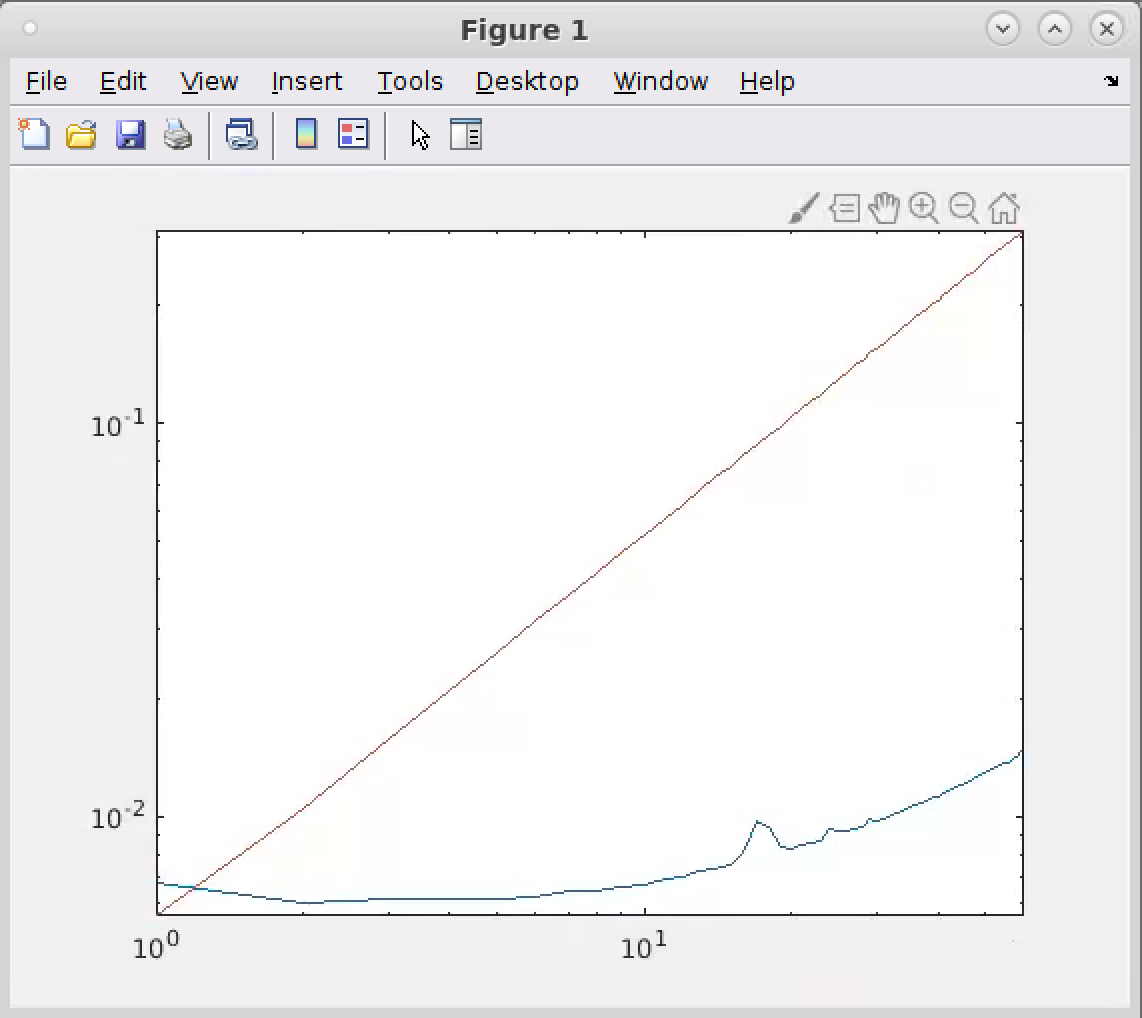
\includegraphics [scale = .5] {TimeGraph}

\end{document}